%%%%%%%%%%%%%%%%%%%%%%%%%%%%%%%%%%%%%%%%%%%%%%%%%%%%%%%%%%%%%%%%%%%%%%
% LaTeX Template: Curriculum Vitae
%
% Source: http://www.howtotex.com/
% Feel free to distribute this template, but please keep the
% referal to HowToTeX.com.
% Date: July 2011
% 
%%%%%%%%%%%%%%%%%%%%%%%%%%%%%%%%%%%%%%%%%%%%%%%%%%%%%%%%%%%%%%%%%%%%%%
% How to use writeLaTeX: 
%
% You edit the source code here on the left, and the preview on the
% right shows you the result within a few seconds.
%
% Bookmark this page and share the URL with your co-authors. They can
% edit at the same time!
%
% You can upload figures, bibliographies, custom classes and
% styles using the files menu.
%
% If you're new to LaTeX, the wikibook is a great place to start:
% http://en.wikibooks.org/wiki/LaTeX
%
%%%%%%%%%%%%%%%%%%%%%%%%%%%%%%%%%%%%%%%%%%%%%%%%%%%%%%%%%%%%%%%%%%%%%%
\documentclass[paper=a4,fontsize=11pt]{scrartcl} % KOMA-article class
							
\usepackage[english]{babel}
\usepackage[utf8x]{inputenc}
\usepackage[protrusion=true,expansion=true]{microtype}
\usepackage{amsmath,amsfonts,amsthm}     % Math packages
\usepackage{graphicx}                    % Enable pdflatex
\usepackage[svgnames]{xcolor}            % Colors by their 'svgnames'
\usepackage{geometry}
	\textheight=700px                    % Saving trees ;-)
\usepackage{url}

\frenchspacing              % Better looking spacings after periods
\pagestyle{empty}           % No pagenumbers/headers/footers

%%% Custom sectioning (sectsty package)
%%% ------------------------------------------------------------
\usepackage{sectsty}

\sectionfont{%			            % Change font of \section command
	\usefont{OT1}{phv}{b}{n}%		% bch-b-n: CharterBT-Bold font
	\sectionrule{0pt}{0pt}{-5pt}{3pt}}

%%% Macros
%%% ------------------------------------------------------------
\newlength{\spacebox}
\settowidth{\spacebox}{8888888888}			% Box to align text
\newcommand{\sepspace}{\vspace*{1em}}		% Vertical space macro

\newcommand{\MyName}[1]{ % Name
		\Huge \usefont{OT1}{phv}{b}{n} \hfill #1
		\par \normalsize \normalfont}
		
\newcommand{\MySlogan}[1]{ % Slogan (optional)
		\large \usefont{OT1}{phv}{m}{n}\hfill \textit{#1}
		\par \normalsize \normalfont}

\newcommand{\NewPart}[1]{\section*{\uppercase{#1}}}

\newcommand{\PersonalEntry}[2]{
		\noindent\hangindent=2em\hangafter=0 % Indentation
		\parbox{\spacebox}{        % Box to align text
		\textit{#1}}		       % Entry name (birth, address, etc.)
		\hspace{1.5em} #2 \par}    % Entry value

\newcommand{\SkillsEntry}[2]{      % Same as \PersonalEntry
		\noindent\hangindent=2em\hangafter=0 % Indentation
		\parbox{\spacebox}{        % Box to align text
		\textit{#1}}			   % Entry name (birth, address, etc.)
		\hspace{1.5em} #2 \par}    % Entry value	
		
\newcommand{\EducationEntry}[4]{
		\noindent \textbf{#1} \hfill      % Study
		\colorbox{Black}{%
			\parbox{6em}{%
			\hfill\color{White}#2}} \par  % Duration
		\noindent \textit{#3} \par        % School
		\noindent\hangindent=2em\hangafter=0 \small #4 % Description
		\normalsize \par}

\newcommand{\WorkEntry}[4]{				  % Same as \EducationEntry
		\noindent \textbf{#1} \hfill      % Jobname
		\colorbox{Black}{\color{White}#2} \par  % Duration
		\noindent \textit{#3} \par              % Company
		\noindent\hangindent=2em\hangafter=0 \small #4 % Description
		\normalsize \par}

%%% Begin Document
%%% ------------------------------------------------------------

\begin{document}
% you can upload a photo and include it here...
%\begin{wrapfigure}{l}{0.5\textwidth}
%	\vspace*{-2em}
%		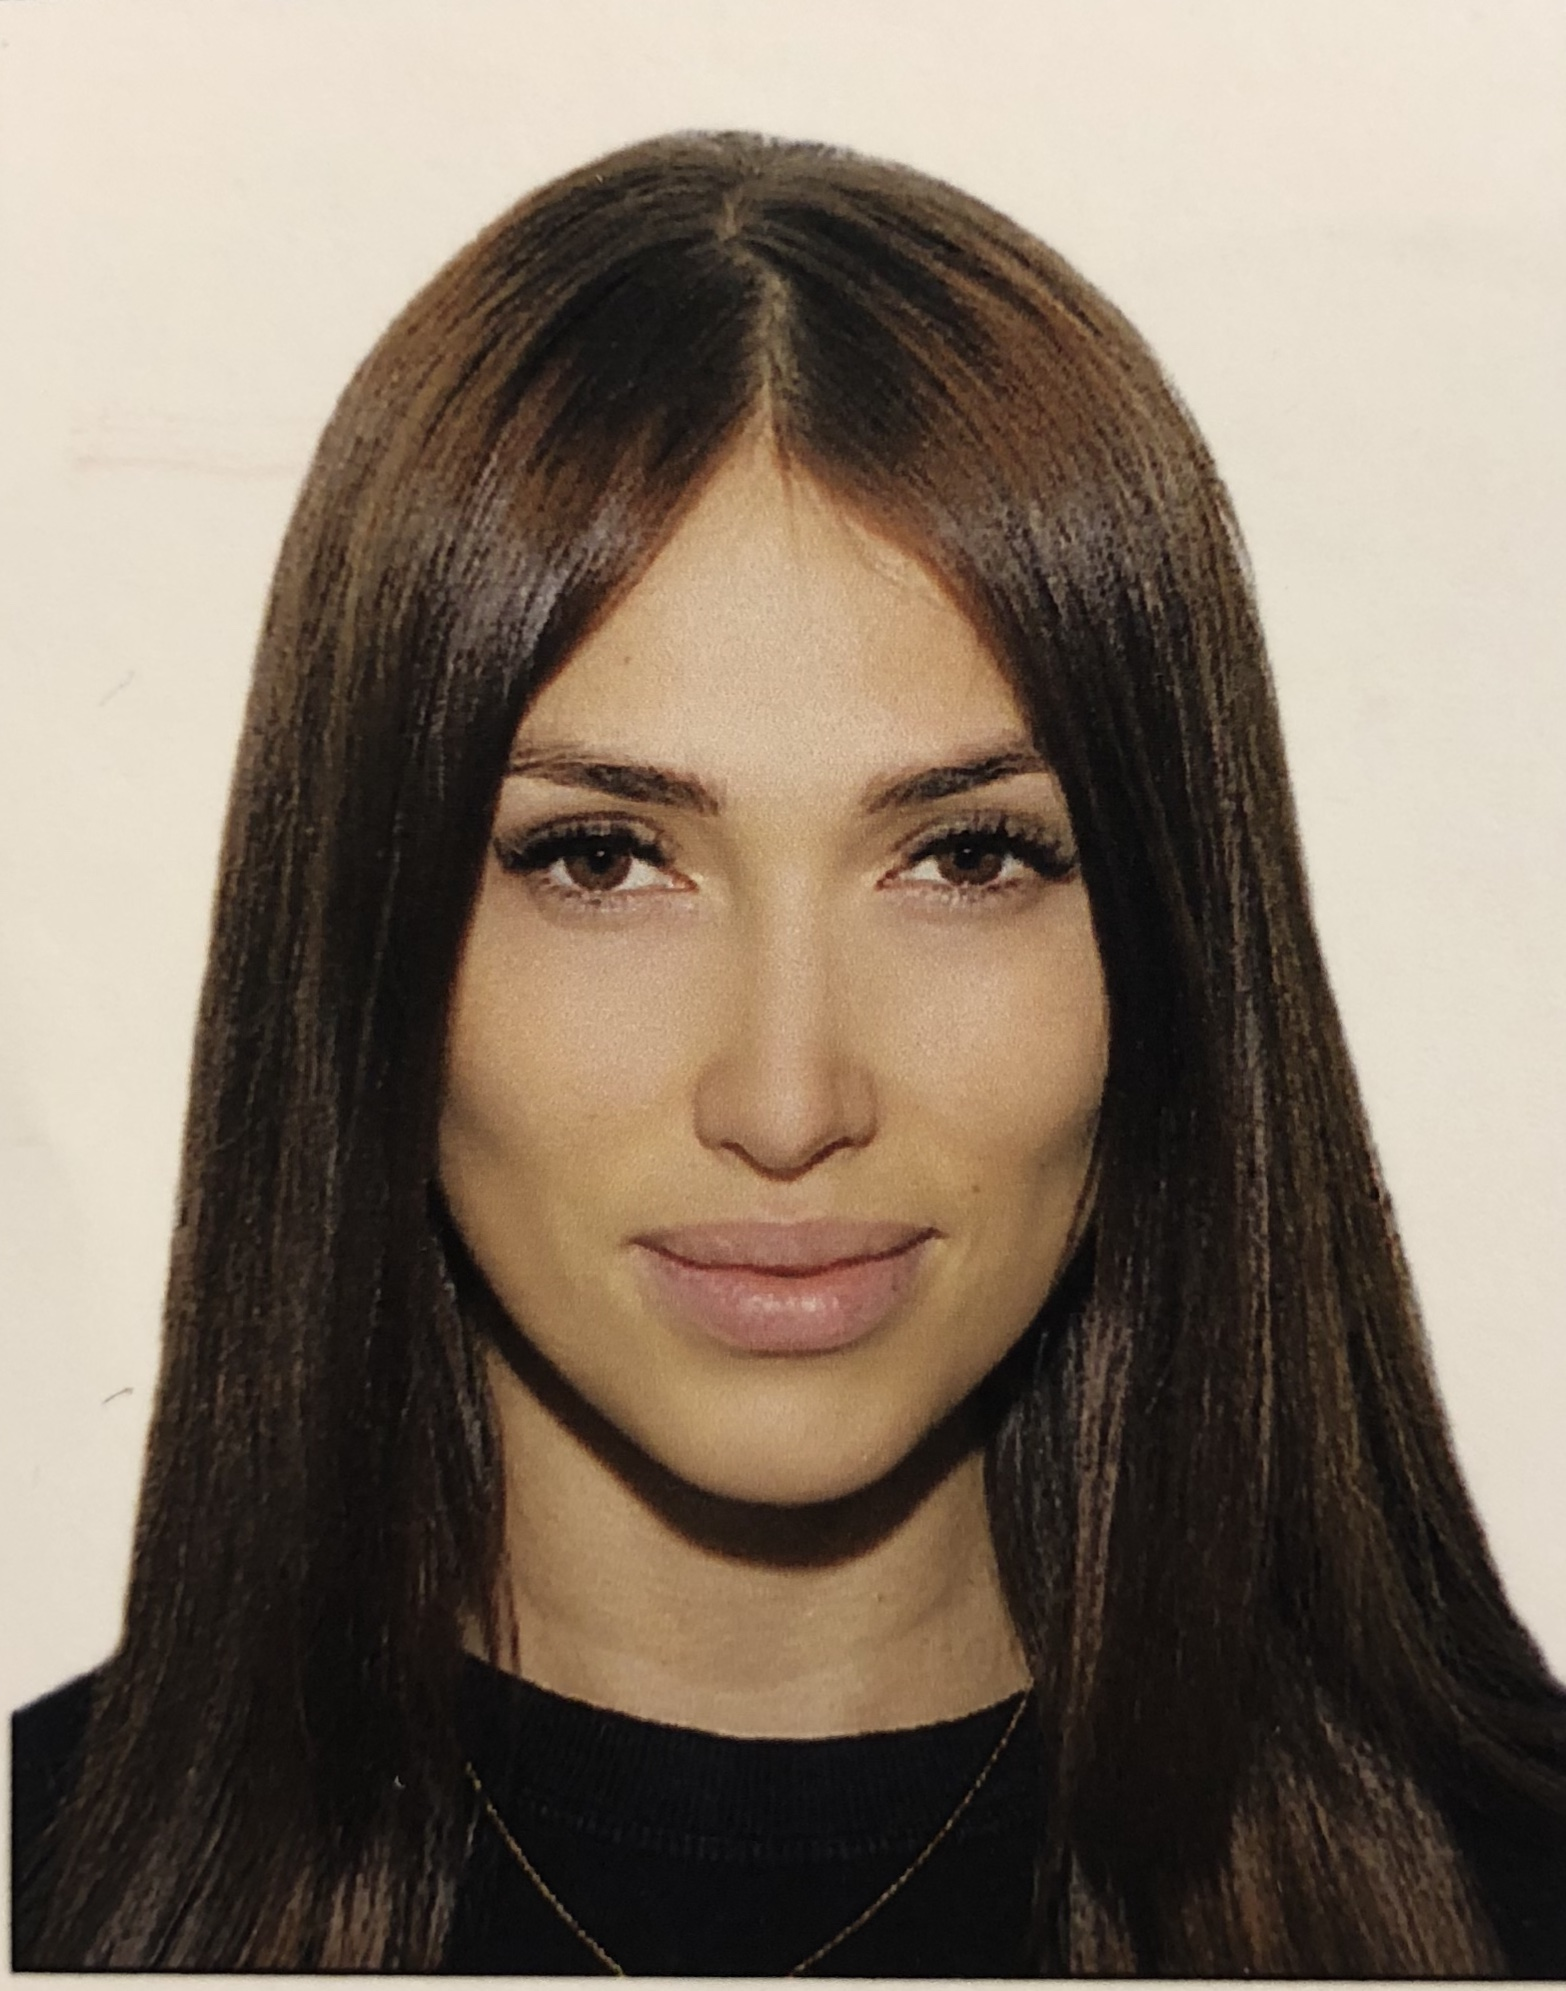
\includegraphics[width=0.15\textwidth]{photo}
%\end{wrapfigure}

\MyName{NAVNEET PANDEY}
%\MySlogan{Indian Institute of Engineering Science and Technology,Shibpur}
\MySlogan{M.Tech. in Electrical Engineering}

\sepspace

%%% Personal details
%%% ------------------------------------------------------------
\NewPart{Personal details}{}

\PersonalEntry{Birth}{January 05, 1994}
\PersonalEntry{Address}{kadipur, Sultanpur Uttar Pradesh 228145}
\PersonalEntry{Phone}{+91-9654961533}
\PersonalEntry{E-mail}{\url{navneetpandey94@gmail.com}}
\PersonalEntry{}{\url{navneetpandey.eee17@itbhu.ac.in}}

%%% Education
%%% ------------------------------------------------------------
\NewPart{Education}{}

\EducationEntry{M.Tech. Indian Institute of Technology,Varanasi }{2017-2019}{Secured 8.34  CGPA.}

\sepspace

\EducationEntry{B.Tech. Greater Noida Institute of Technology greater Noida}{2011-2015}{Secured 73.34 percentage.}

\sepspace

\EducationEntry{12th SVM Inter College}{2008-2010}{Uttar Pradesh Board of
Higher Education}{Secured 78.20\% marks in 12th standard.}
\sepspace

\EducationEntry{10th SVM Inter College}{2008}{Uttar Pradesh Board of
Secondary Education}{Secured 64.50\% marks in 10th standard.}

%%% Work experience
%%% ------------------------------------------------------------
\NewPart{INTERNSHIPS}{}

\WorkEntry{Industrial Training}{may 14- july 14}{IPGCL, New Delhi}{Title : Relational inductive biases, deep learning, and graph networks\\Supervision : Under Dr. Malay Bhattacharyya, ISI, Kolkata\\About : Analyzing the neural networks to operate on graphs.}
\sepspace

\WorkEntry{Summer Internship}{May'13-June'13}{Logicon Automation Lucknow}{Title : Overview of PLC SCADA and thier programming\\Supervision : Under Dr. Malay Bhattacharyya, ISI, Kolkata\\About : In this research work, we statistically analyzed how the miRNAs are related to Cancer causing
mutations.}

%%% project
%%% ------------------------------------------------------------
\NewPart{Projects}{}

\WorkEntry{M.Tech Project}{July'18-June'19}{Direct Torque Control of Induction Motor}{Supervision : Under Dr. N K Swami Naidu, IIT BHU, Varanasi\\We have developed a Network-On-Chip simulator, Noxim. Our main objective was \\to develop a simulator that can perform all types of functionalities in a single platform.}
\sepspace


\WorkEntry{Personal Project}{June'18-July'18}{Supervision : Under Dr. Santi P. Maity, IIEST, Shibpur\\Gold Code generation using 255 bit PN Generator and Multi-User Detection}{In this project we had designed a Gold Code Generator using two 255 bit PN Generator and analyzed its
properties.}
\sepspace


\WorkEntry{Personal Project}{Dec'17-present}{Supervision : Under Dr. Prasun Ghosal, IIEST, Shibpur\\Online Compiler and data storage}{I am working on a website from where anyone can take help for their coding, they can upload their codes
there, they can compile codes. If anyone wants to ask for help for particular purpose they can post their
problem statement there.}





\NewPart{Certifications}{}

\WorkEntry{PHP with MySQL}{}{Aspirevision Tech, Microsoft}{}
\sepspace
\WorkEntry{Cloud Computing}{}{Electrocloud Labs of NIT Durgapur}{}

%%% Skills
%%% ------------------------------------------------------------
\NewPart{Skills}{}

\SkillsEntry{Languages}{Bengali (mother tongue)}
\SkillsEntry{}{English}
\sepspace

\SkillsEntry{Programming Languages}{\textsc{C/C++}, \textsc{Python}, \textsc{PHP}, \textsc{Java}, \textsc{VHDL}}
%\SkillsEntry{}{Python}
%\SkillsEntry{}{PHP}
%\SkillsEntry{}{Java}
%\SkillsEntry{}{VHDL}
\sepspace

\SkillsEntry{Software}{\textsc{Matlab}, \textsc{Xilinx ISE}, \textsc{Bioinformatics}, \textsc{SystemC}}
\sepspace


\SkillsEntry{Subjects}{\textsc{Compiler Designing}, \textsc{Computer Nteworks}, \textsc{Algorithms}}
\SkillsEntry{}{\textsc{Operaing
System}, \textsc{DBMS}, \textsc{Microprocessor}}
\SkillsEntry{}{\textsc{Computer Architecture and Organisation }, \textsc{Graphics}}
\SkillsEntry{}{\textsc{Automata Theory and Natural Languages}}
\SkillsEntry{}{\textsc{Signals Systems and Circuits}, \textsc{Data Structures}}
\SkillsEntry{}{\textsc{Discrete Mathematics}, \textsc{Communication Systems}}
\SkillsEntry{}{\textsc{Digital Logic and Circuit Design}}


%%% References, 
%%% ------------------------------------------------------------
\NewPart{Extra Curricular Activities}{}
%Available upon request
1. Member of Society of Information Technology, IIEST, Shibpur
\\
\sepspace
2. Swimming
\end{document}
